\section{Mobile client}

As described in \cref{sub:smartphone_usage} and \cref{pact}, execution
of an request should be quick and easy to navigate an use, to minimise
the time spend using the system. Throughout this section the
guidelines described in \citetitle{DEB} will be followed.

\subsection{Navigation}

Users build mental navigation maps of the systems they are using, and
they tend to keep using already memorised paths to certain views~\cite{DEB}.

A recommendation to achieve this is that the user should always be able to find \emph{home}, where the user started navigating, from every possible window of the system. This was achieved by having a home button in the top left corner, that always returns to home.

Another recommendation is to provide a simple and short path to all views. This
was achieved by making all views accessible from home. See \cref{fig:UserInterface}.

\begin{figure}[hbtp]
  \centering
  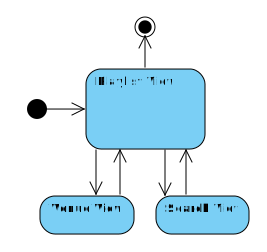
\includegraphics[width=0.5\textwidth]{Images/UserInterface.pdf}
  \caption{Diagram of navigation in the user interface.}\label{fig:UserInterface}
\end{figure}

\begin{itemize}
\item Venue view: The user is presented a list of venues for the user to check in at, see \cref{fig:VenueSketch}.
\item Playlist view: The user is now checked in at a venue and is presented with the playlist of the venue, including what is current playing. See \cref{fig:PlaylistSketch}.
\item Search view: From here the user can search for a track in the music catalogue. The search bar is indicated by a magnifying glass, See \cref{fig:SearchSketch}. When results of the search query is received from the server, is it displayed below the search bar, in descending order according to relevance.
\end{itemize}

The idea behind the \emph{+} icon in the top right of \cref{fig:PlaylistSketch}, is that it should indicate a process of "adding", in this context adding to the playlist. During some usability tests this was shown to be viable assumption, in that this was not a cause to any of the problems found, the usability tests will be described in \cref{sub:usabilityTesting}.
Should the user want to change venue, one is checked in at, another list view of venue \enquote{swiped} in from the left. Following the reading direction of left to right, giving a notion of upper layered list of venues, from which the user can change between lower layered playlists.

\begin{figure}[hbtp]
  \centering
  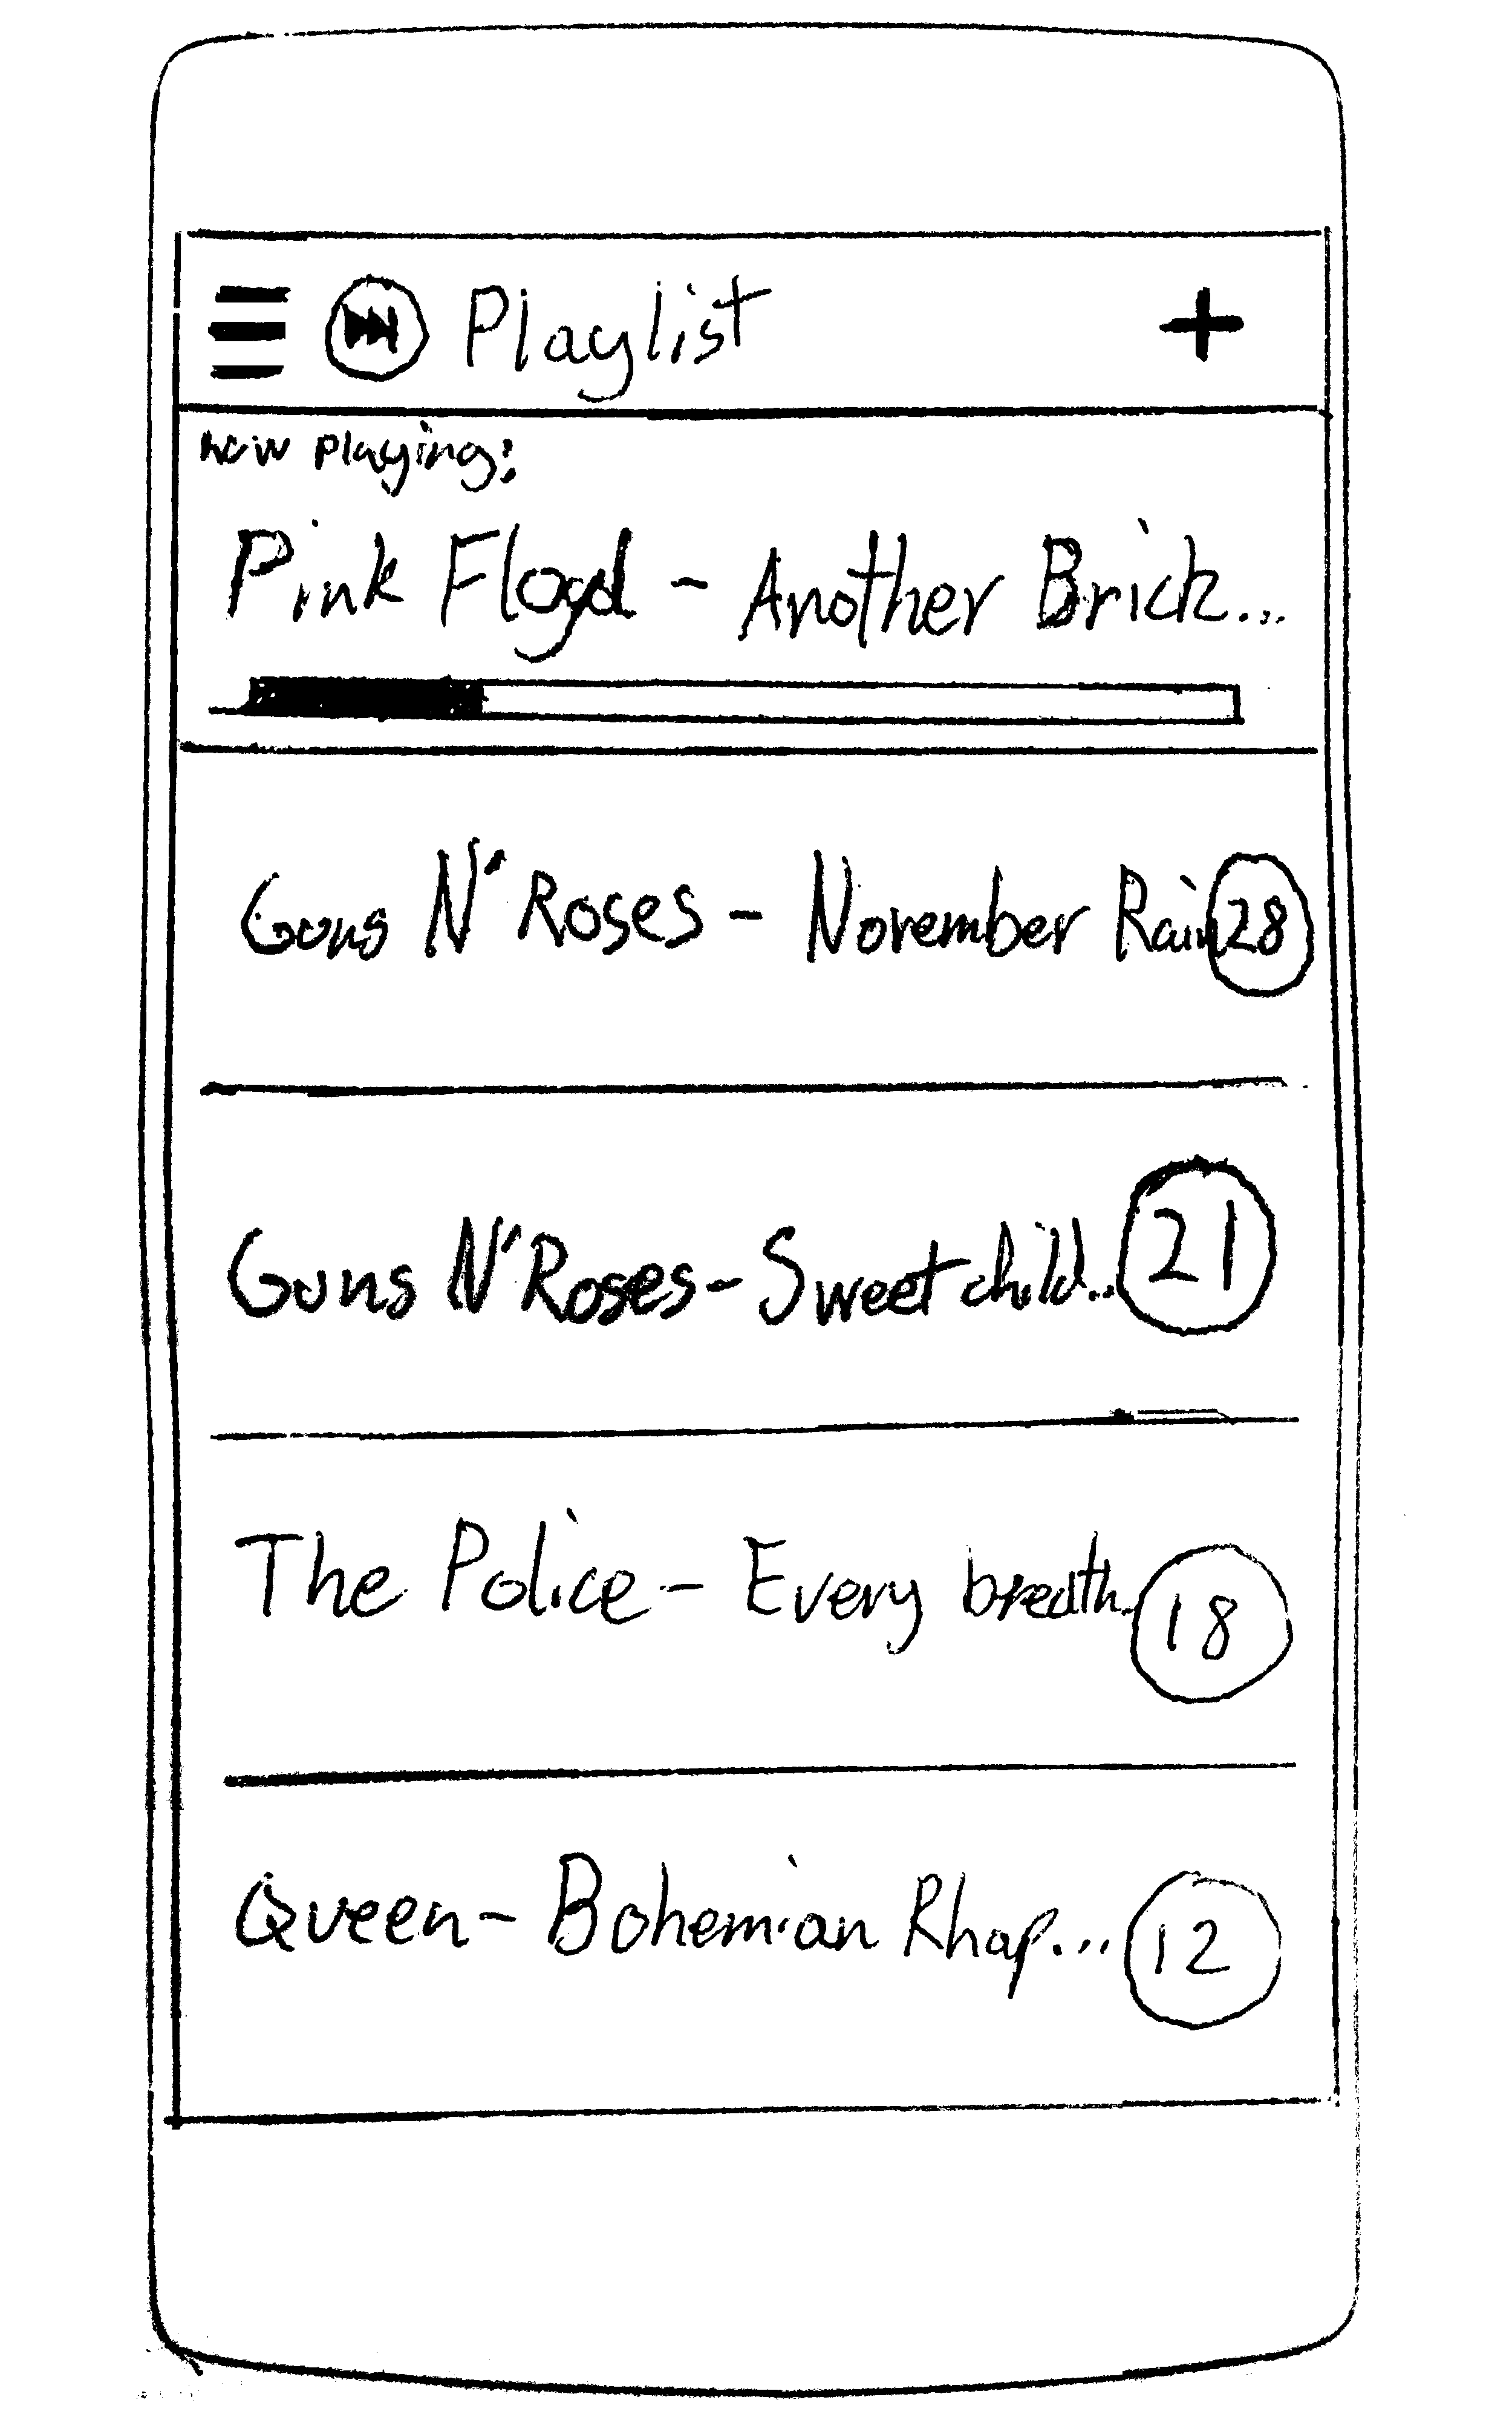
\includegraphics[width=0.3\linewidth]{Images/sketch3.png}
  \caption[Playlist view sketch.]{This view presents the user with the current playlist.}
  \label{fig:PlaylistSketch}
\end{figure}

\begin{figure}[hbtp]
  \centering
  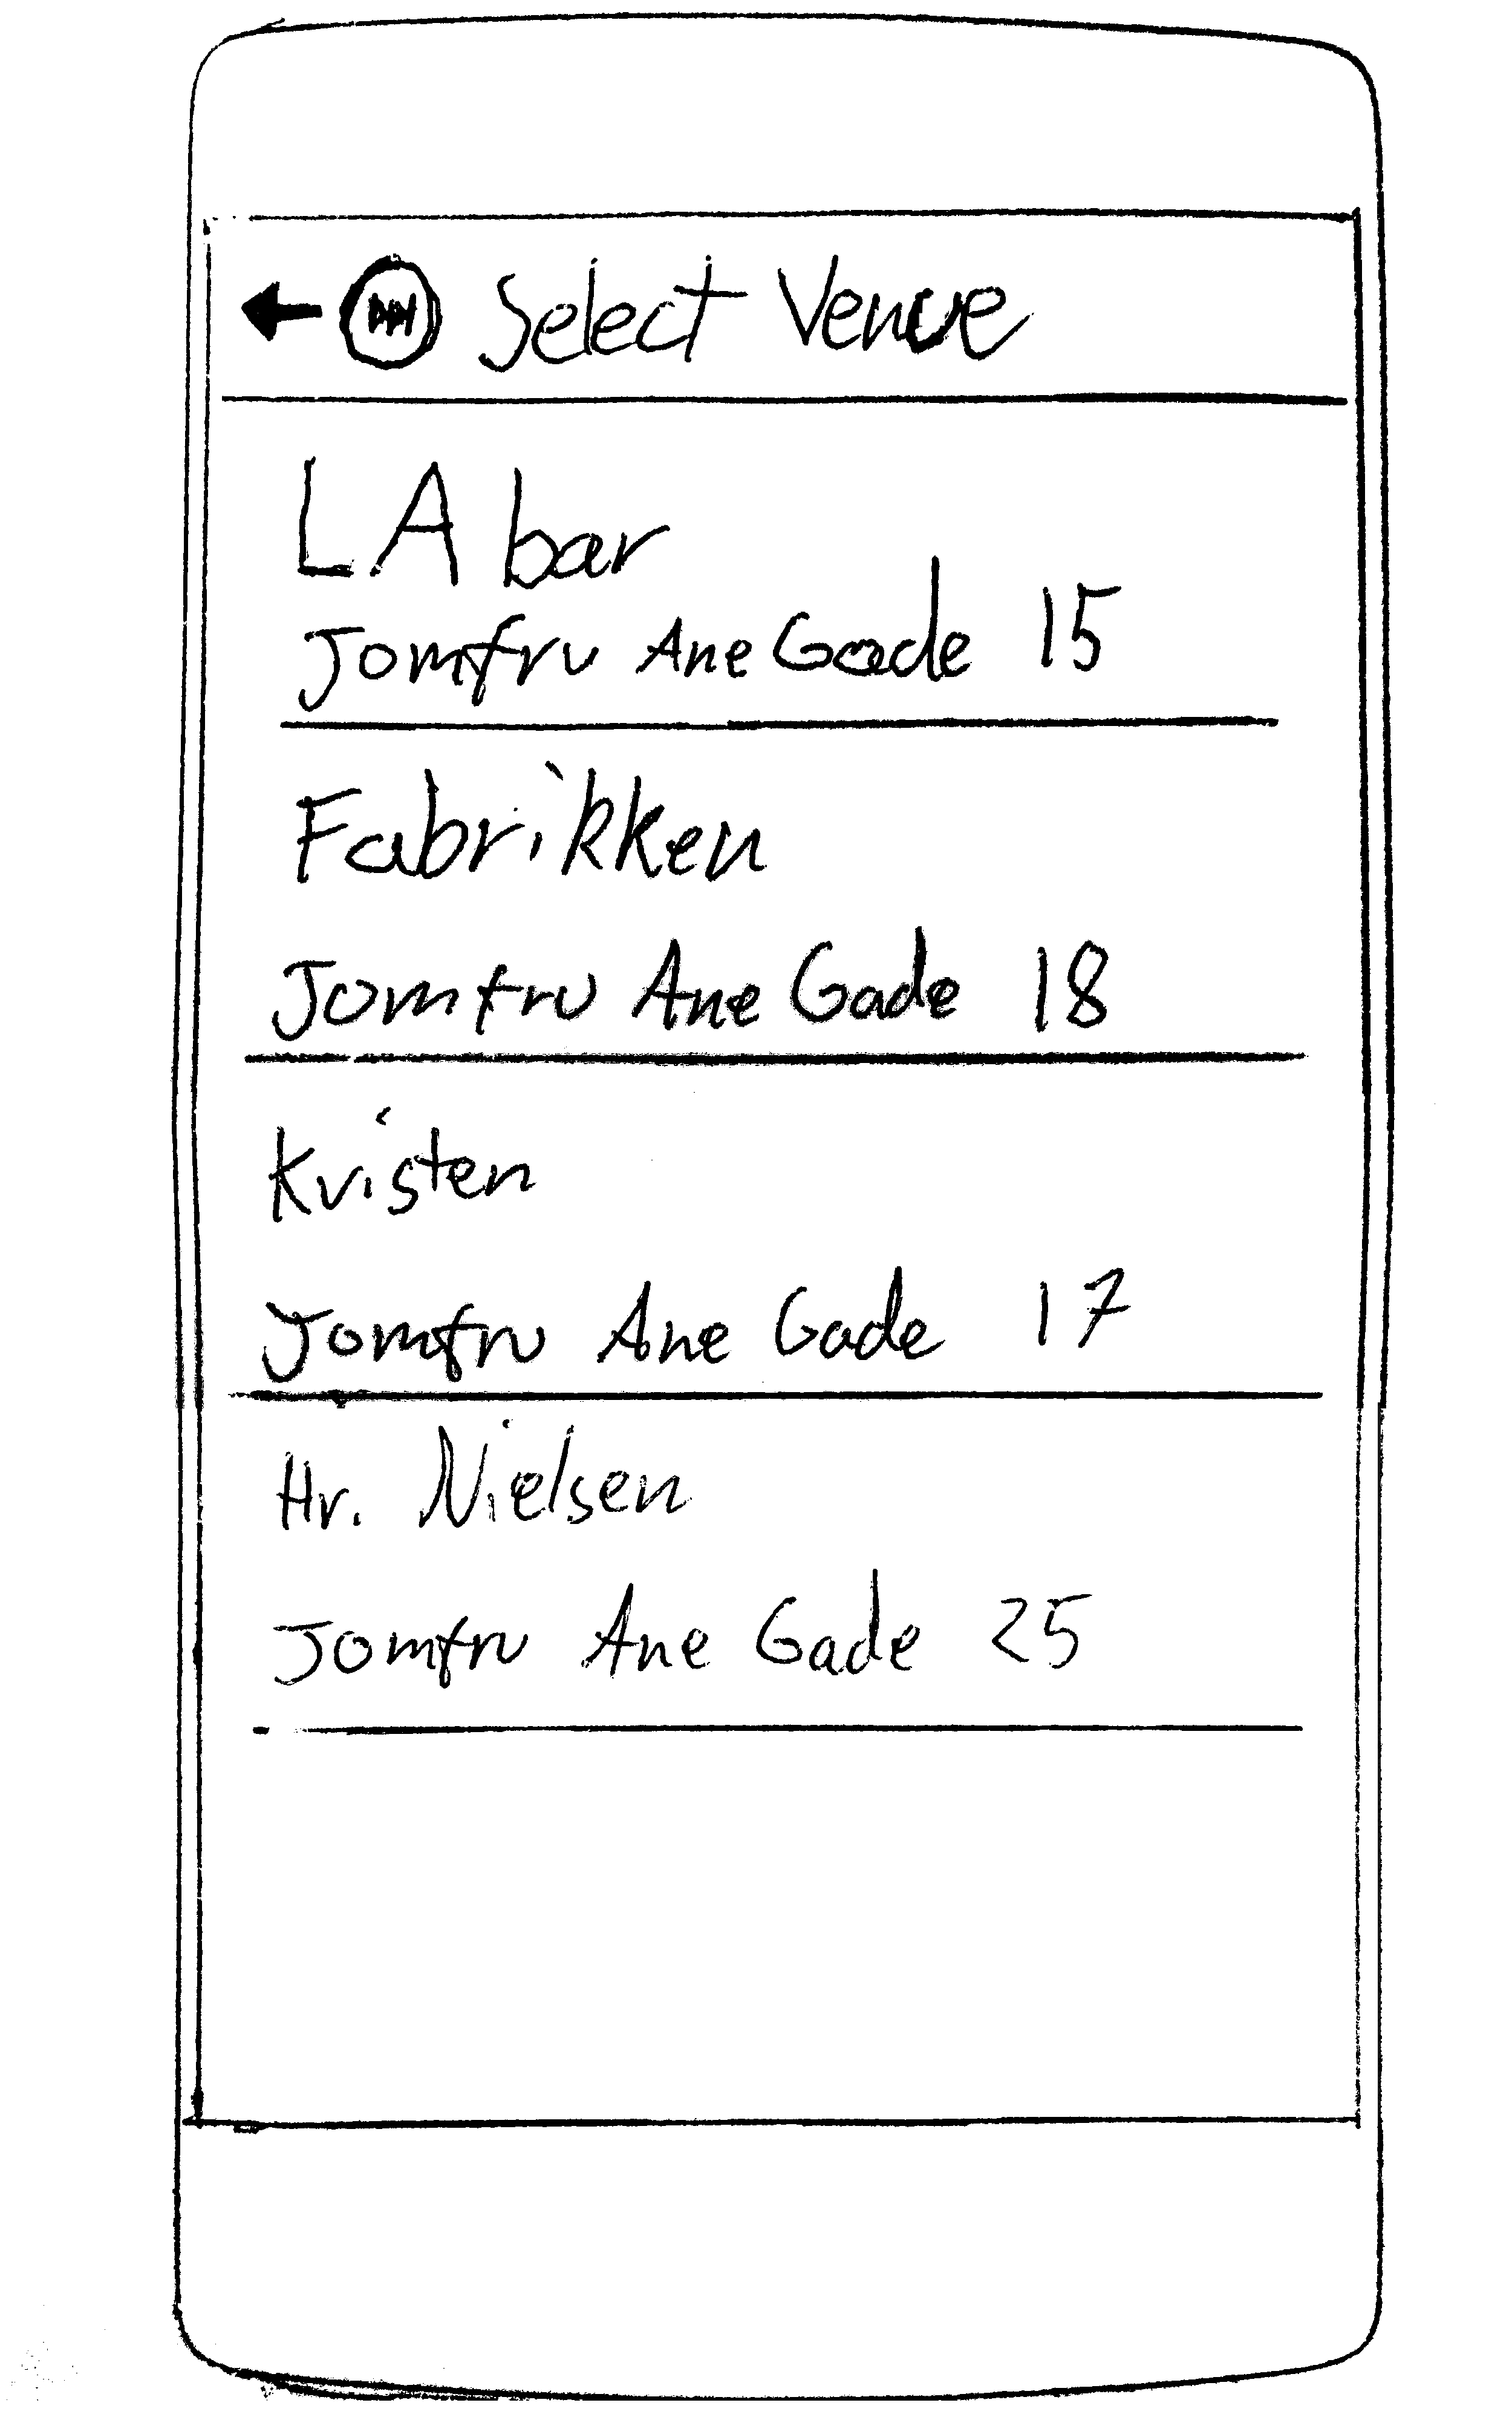
\includegraphics[width=0.3\linewidth]{Images/sketch2.png}
  \caption[Venue view sketch.]{The user can see a listing of nearby open venues. The user can click on any one of these to check in to the venue.}
  \label{fig:VenueSketch}
\end{figure}


\begin{figure}[hbtp]
  \centering
  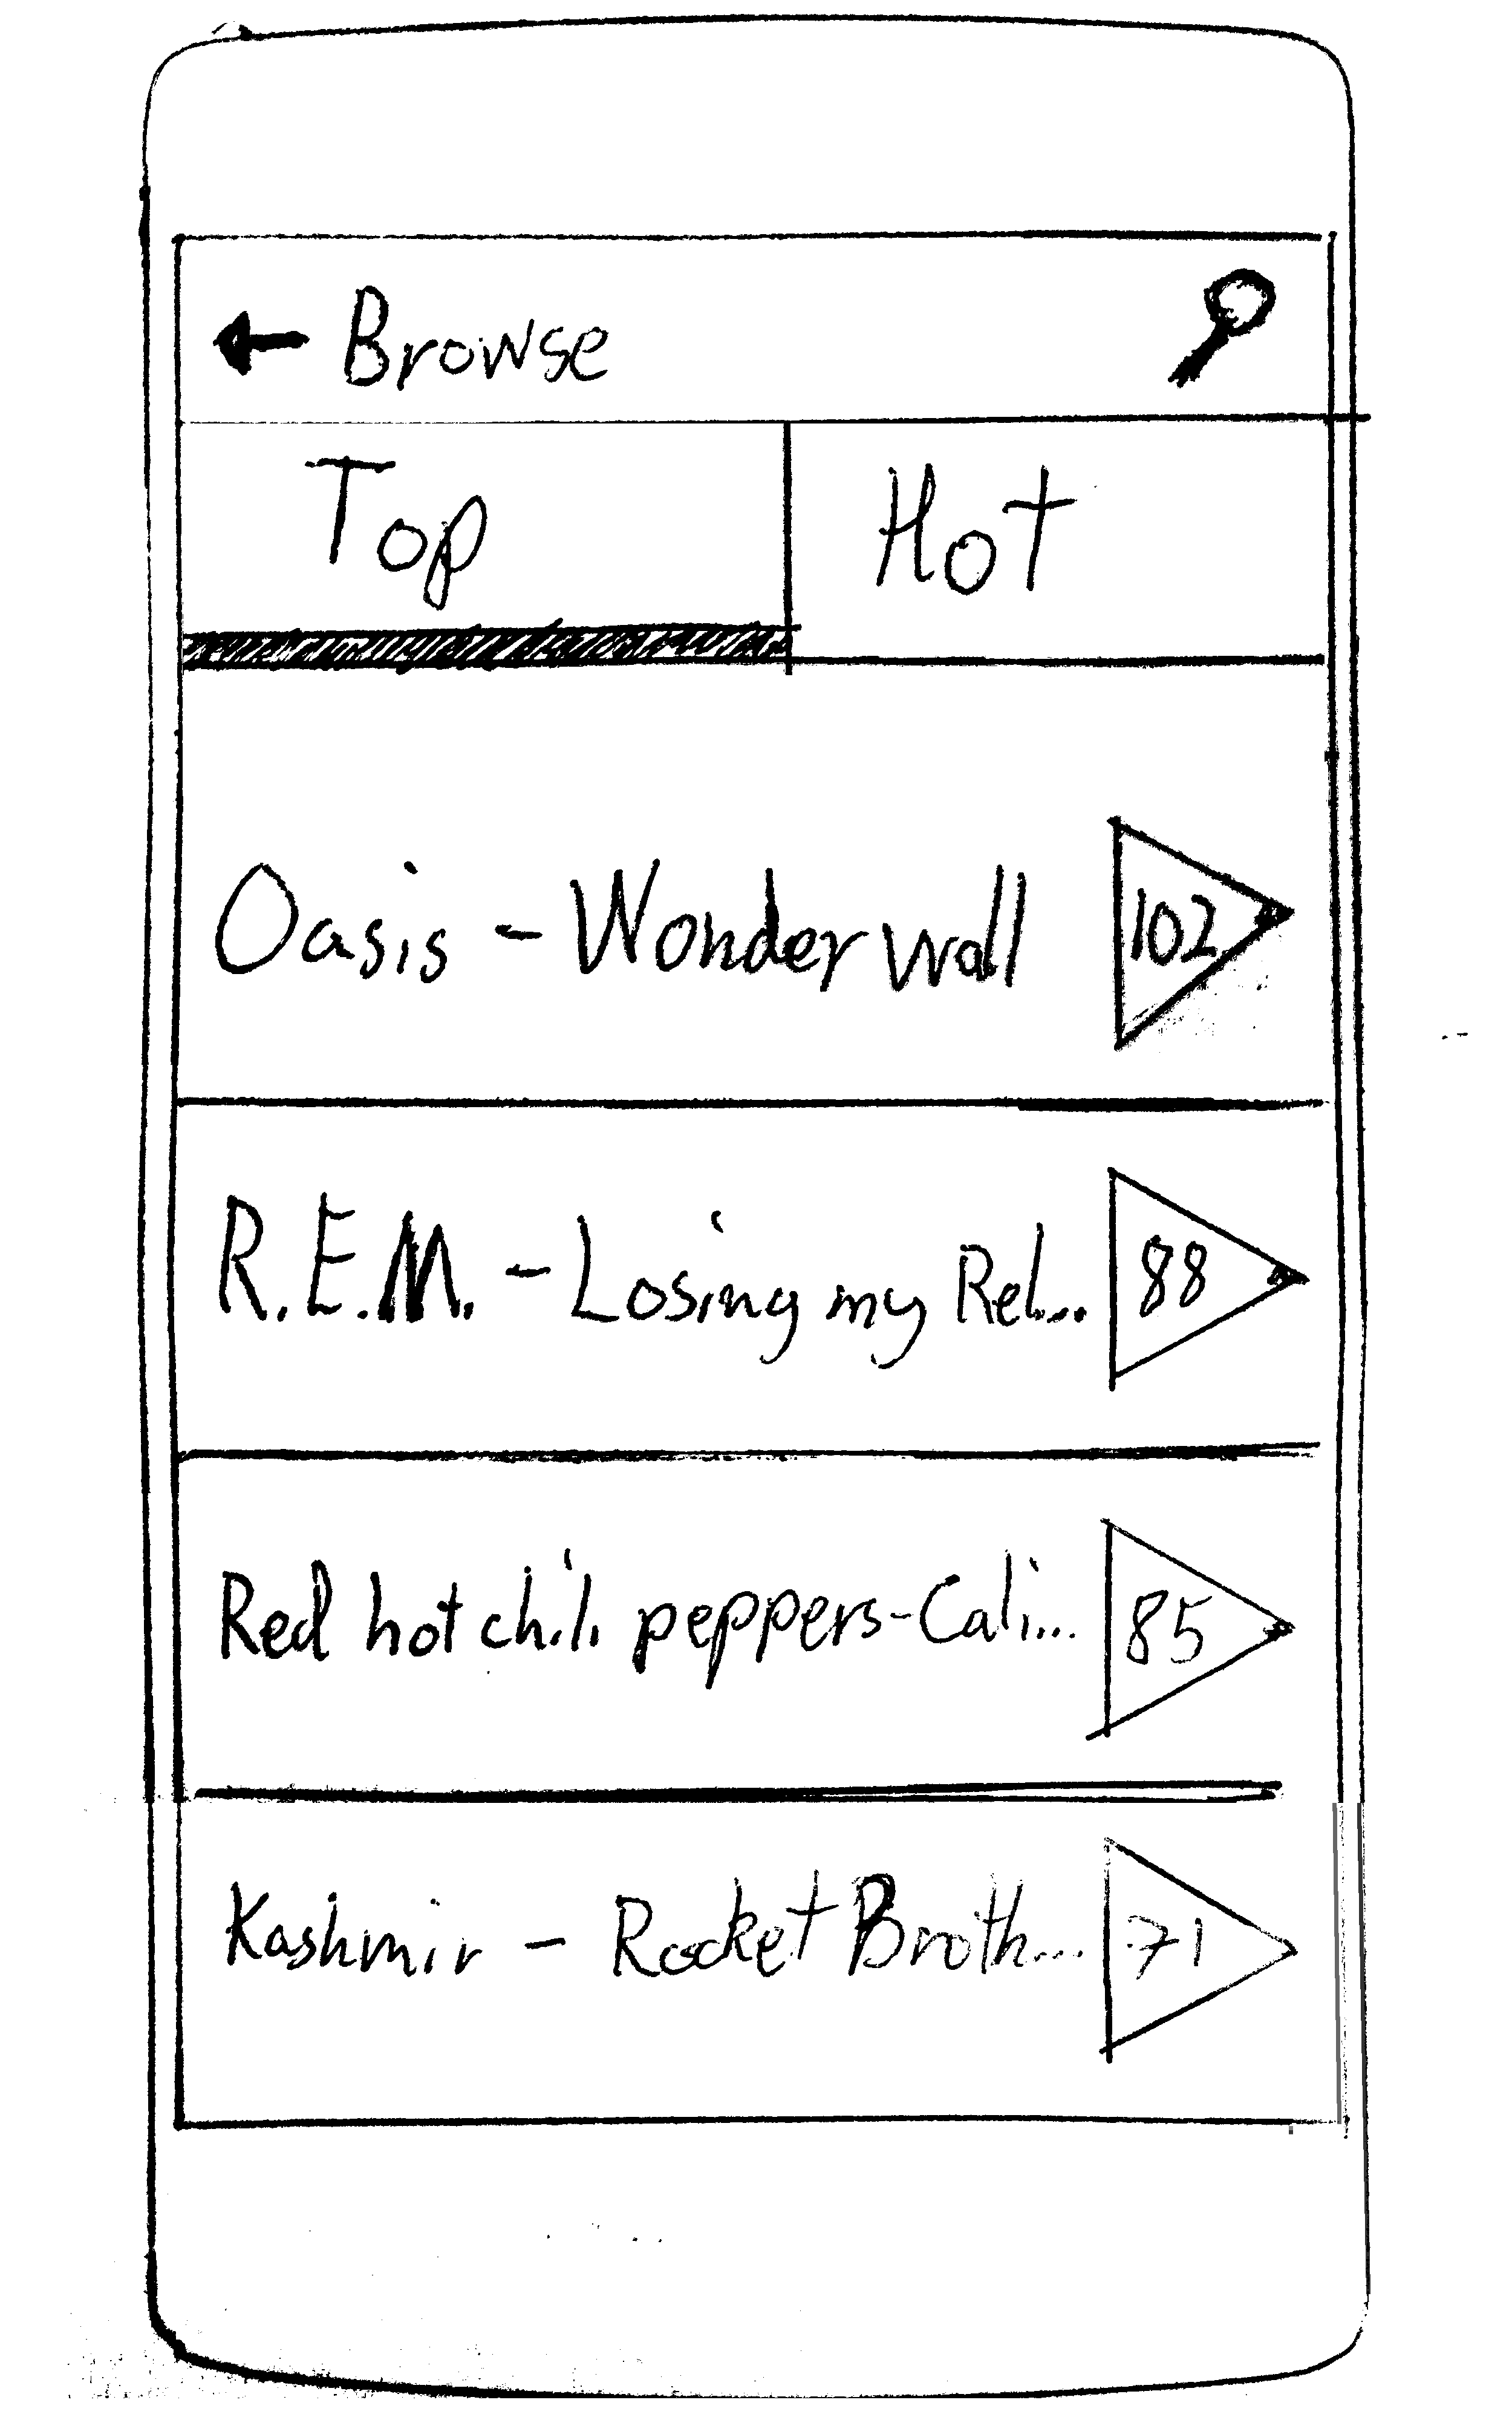
\includegraphics[width=0.3\linewidth]{Images/sketch4.png}
  \caption[Search sketch.]{The magnifying glass at the very top is symbolising an action of searching, when clicked the user can search for specific tracks.}
  \label{fig:SearchSketch}
\end{figure}

From \cref{sub:usabilityTesting} it was extracted that the interface should change views automatically as a confirmation of an action completed. This resulted in when selecting a venue in the venue view or a track in the search view, the user would be presented with the current playlist of the venue, at the playlist view.
